
\section{Introduction}

Minimum cost path is a classical problem in computer science. This problem has many variations but often uses a 2D matrix/grid representation: given an $M \times N$ matrix, source cell $S$, and destination cell $D$, find the shortest distance from $S$ to $D$ by moving up, down, left, and right to adjacent cells.

% \begin{figure}[h]
%     \centering
%     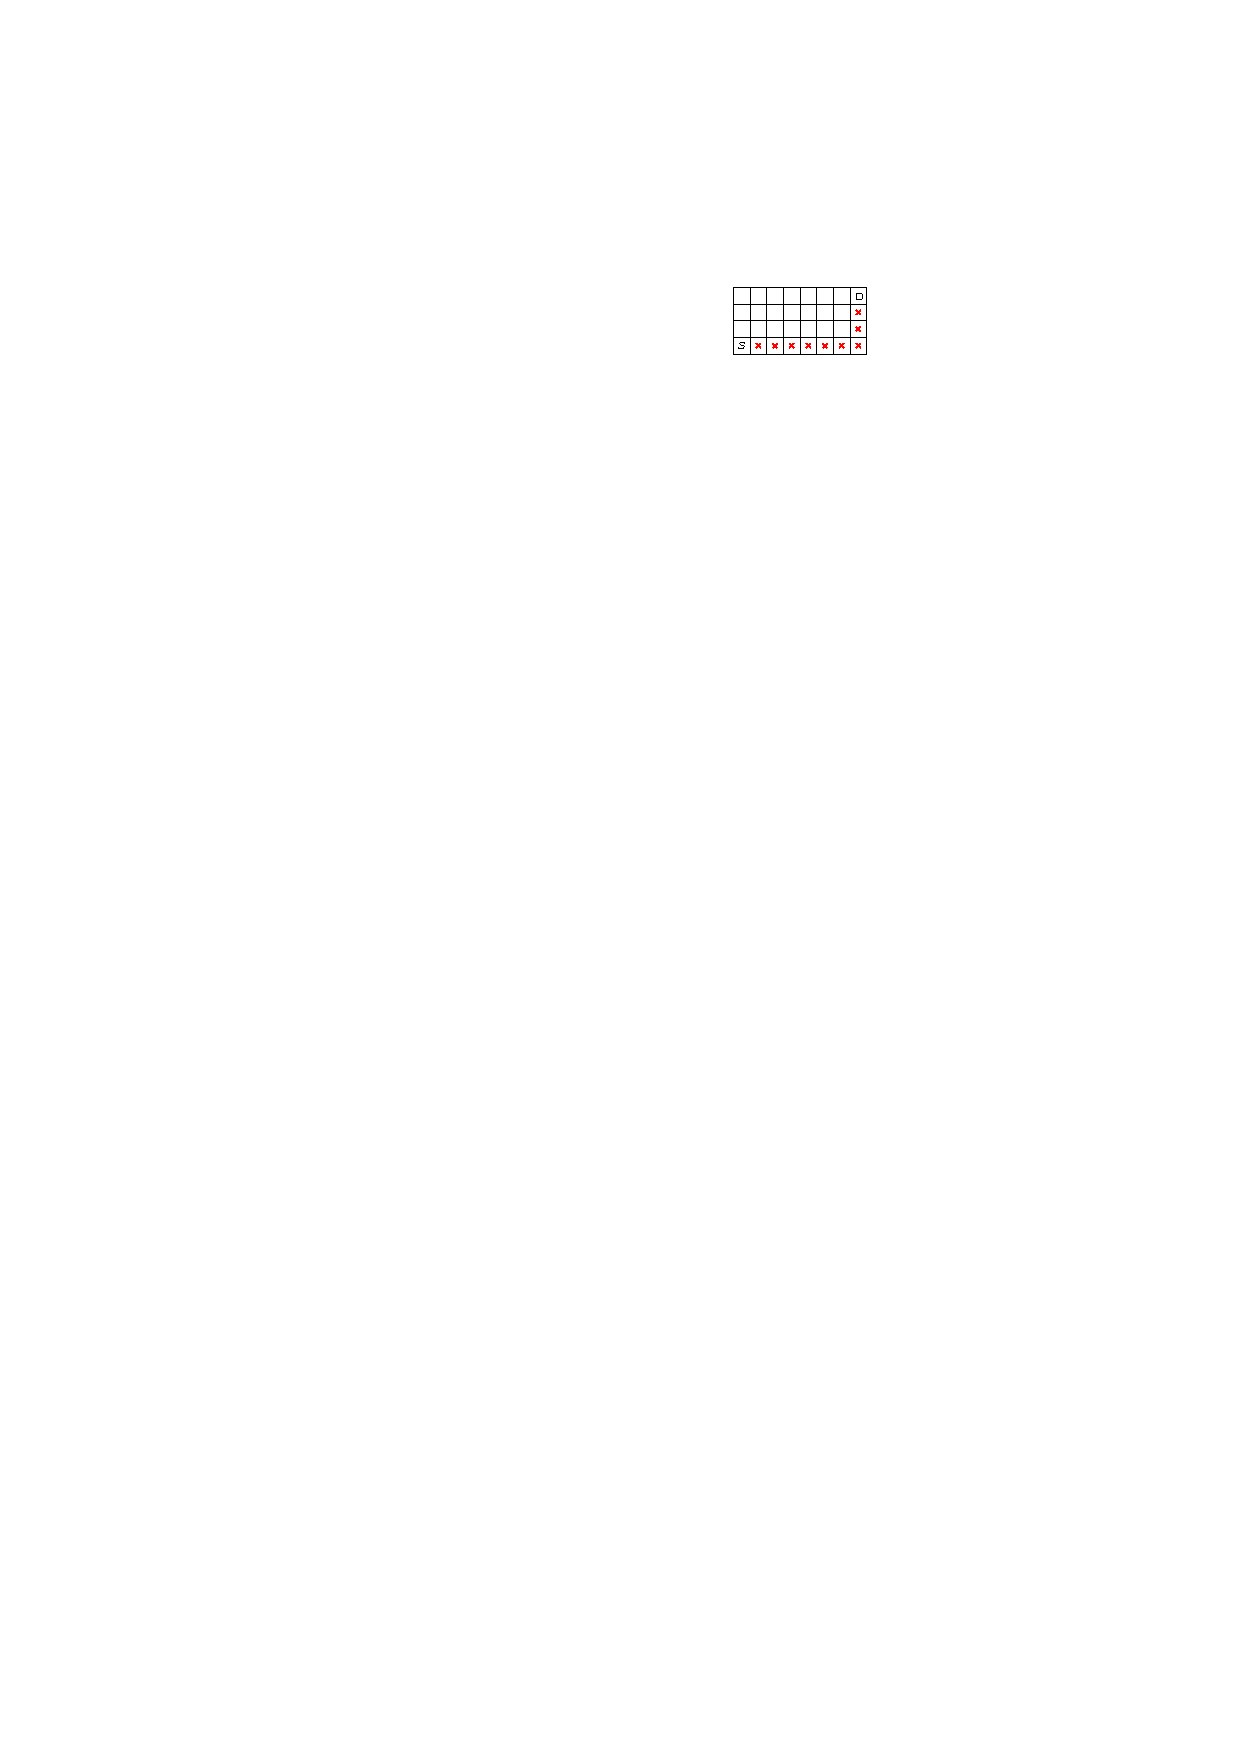
\includegraphics[scale=2]{figures/grid.pdf}
%     \caption{ \small A $4 \times 8$ grid representation with 10 movements. $S=(0,0)$ and $D=(7, 3)$.}
%     \label{fig:basic-grid}
% \end{figure}

A solution to the minimum cost problem is to simply apply either breadth-first or depth-first search from $S$. For any matrix or directed acyclic graph, finding $D$ will trivially yield the shortest path as well. Although finding the minimum cost path for an $M \times N$ matrix can be found in $O(M \times N)$ time using a BFS, we would like to explore the application of an evolutionary algorithm to this problem.

\subsection{Problem Statement}

 For the scope of this work, we add several constraints to the original minimum cost problem.
\begin{enumerate}
    \item Consider only square matrices i.e. $N \times N$ matrices.
    \item $S$ and $D$ are fixed at $(0, 0)$ and $(N-1, N-1)$ respectively. \label{two}
    \item Possible movements from one cell to the next are up, right, diagonal, and none.
    \item All movements between adjacent (including diagonally adjacent) cells incur the same cost.
\end{enumerate}

Constraint (2) implies that $S$ will always be the bottom-leftmost cell and $D$ will always be the upper-rightmost cell. Notice that for any $M \times N$ matrix, every path consisting of $M-1$ movements up and $N-1$ movements to the right will be a minimal path. In fact, if we are to consider only up and right movements between cells, every possible path will be the same length: $M + N - 2$. Therefore, constraint (3) is required to make this problem more interesting. By adding in a diagonal movement, we can reduce the cost of any up and right movement by 1. For any square matrix, the minimal path will always consist of exactly $N-1$ diagonal movements through every cell $(i, i)$. The first diagonal movement goes to $(1,1)$, and the last diagonal movement goes to $(N-1, N-1)$. Figure~\ref{fig:square-grid} shows a square matrix with its optimal path in red.

% \begin{figure}[h]
%     \centering
%     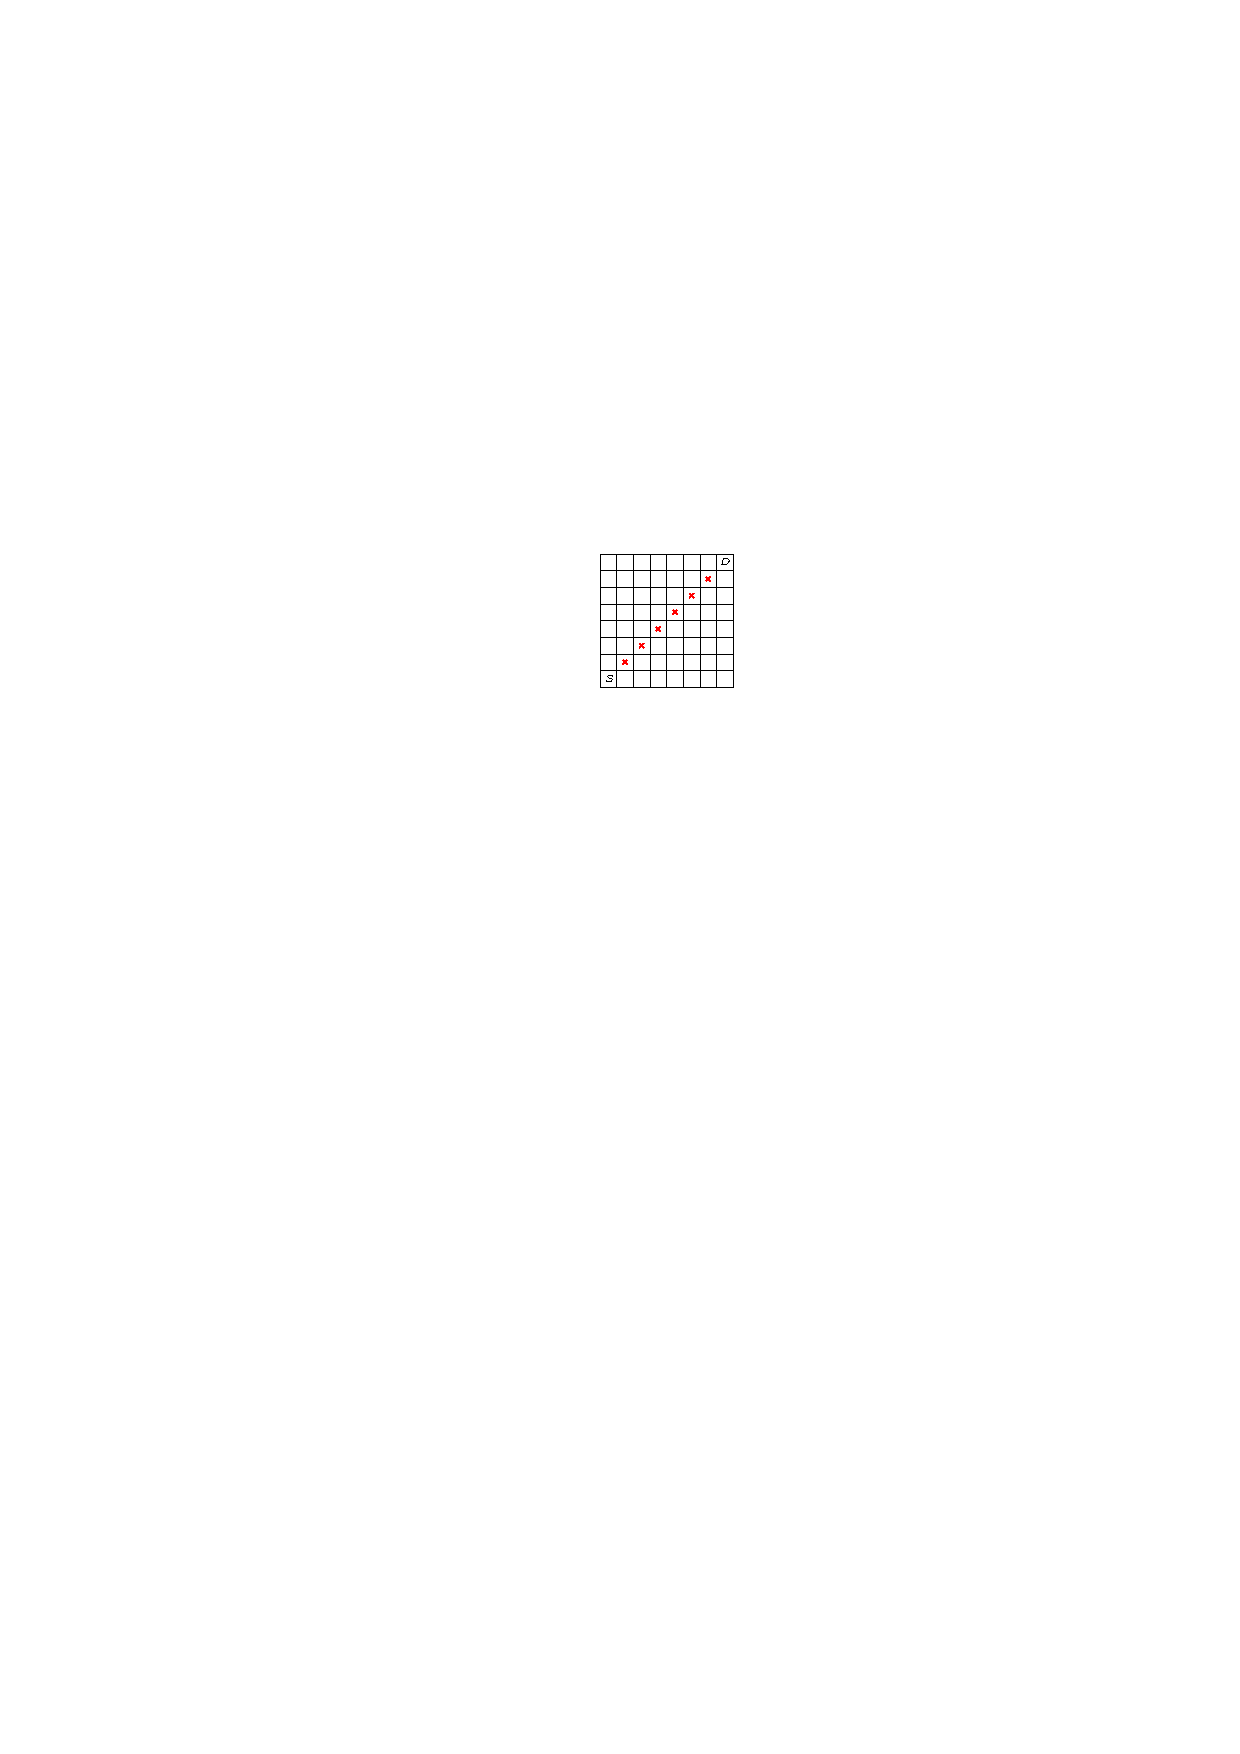
\includegraphics[scale=2]{figures/square_grid.pdf}
%     \caption{ \small An $ 8\times 8$ grid with a 7 move all-diagonal path.}
%     \label{fig:square-grid}
% \end{figure}

Using an evolutionary algorithm, we would like to see a convergence to a path of all diagonals for any arbitrarily sized square matrix in order to solve this version of the minimum cost problem.
